\subsection{Advection-Diffusion Energy Preservation}
\label{sec:advDiff}
Motivated by the fact that in turbulent simulations the preservation of energy at different scales (or wavenumbers) is of paramount importance, we wanted to explore the potential benefit of having sets of families of stable numerical schemes with modifiable dispersion and dissipation properties.

By solving the linear advection-diffusion equation we are able to assess how much dissipation in different scales is due to numerics as opposed to the nature of the equation.

\subsubsection{Setup}

In these numerical experiments we solve the linear advection-diffusion equation using the C1FR and nodal DG schemes following the approach described by Huynh \cite{huynh2009reconstruction}. In essense, we re-write the diffusion-advection equation as a system of two first order \gls{pde}s as follows
\begin{equation}
\begin{split}
\dd{u}{t} + \dd{q}{x} = 0 \\
q - au + \kappa\dd{u}{x} = 0
\end{split}
\end{equation}

where $a$ is the advection speed, $\kappa$ is the diffusion coefficient, and $q$ is a dummy variable. The desired scheme is used to discretize the spatial differentiation.

In this section, we let $a = 1$, $\kappa = 10^{-2}$. The domain was $\Omega = [-10,10]$ and was discretized in $n = 20$ equispaced elements of polynomial order $P = 5$. The boundary conditions were periodic. The initial conditions were sine waves with low, medium, and high wavenumbers. The wavenumbers were chosen relative to the Nyquist limit of the discretization: 
\[k = \rho (P+1)\pi/h\]
 where $\rho$ is a non-dimensional constant, $P+1$ is the number of solution points in each element of polynomial degree $P$, and $h$ is the size of the element. Note that when $\rho = 1$, the Nyquist limit is reached exactly if the solution points are spaced evenly.

In our experiments, for the low wavenumber $\rho = 0.25$; medium wavenumber $\rho = 0.5$; high wavenumber $\rho = 0.75$. The fluxes were all fully upwinded and in the \gls{c1fr} scheme, $c_1 = -5\cdot10^{-3}$. The solution is advanced with a standard \gls{rk}4 time-stepping scheme. A \gls{cfl} of $0.3$ is used for both schemes. At each timestep, we calculate the square of the L-2 norm of the solution and its derivative, and compare it to the exact corresponding values. $||u||_{(2,m)} $ is the L-2 norm of the $m^{\text{th}}$ derivative of solution $u$.


\subsubsection{Results and discussion}
Fig. \ref{fig:low_wavenumber} shows that both schemes preserve the exact solution and derivative norms of the low wavenumber. On the other hand, \ref{fig:high_wavenumber} shows that both schemes suffer from aliasing and deviate significantly from the exact L-2 norms when the initial solution is a high wavenumber. \gls{c1fr} is somewhat closer to the exact values than nodal \gls{dg} both before and after the norms of the numerical solutions intersect the exact solution's L-2 norm.

Fig. \ref{fig:medium_wavenumber} presents a promising result. \gls{c1fr} preserves the correct L-2 norms of the solution while nodal \gls{dg}'s numerical dissipation affects the energy content of the wave. The L-2 norm of C1FR's solution derivative oscillates around the exact value, while nodal \gls{dg}'s oscillates with similar magnitude trending further below the exact values.


\begin{figure}[h]
\centering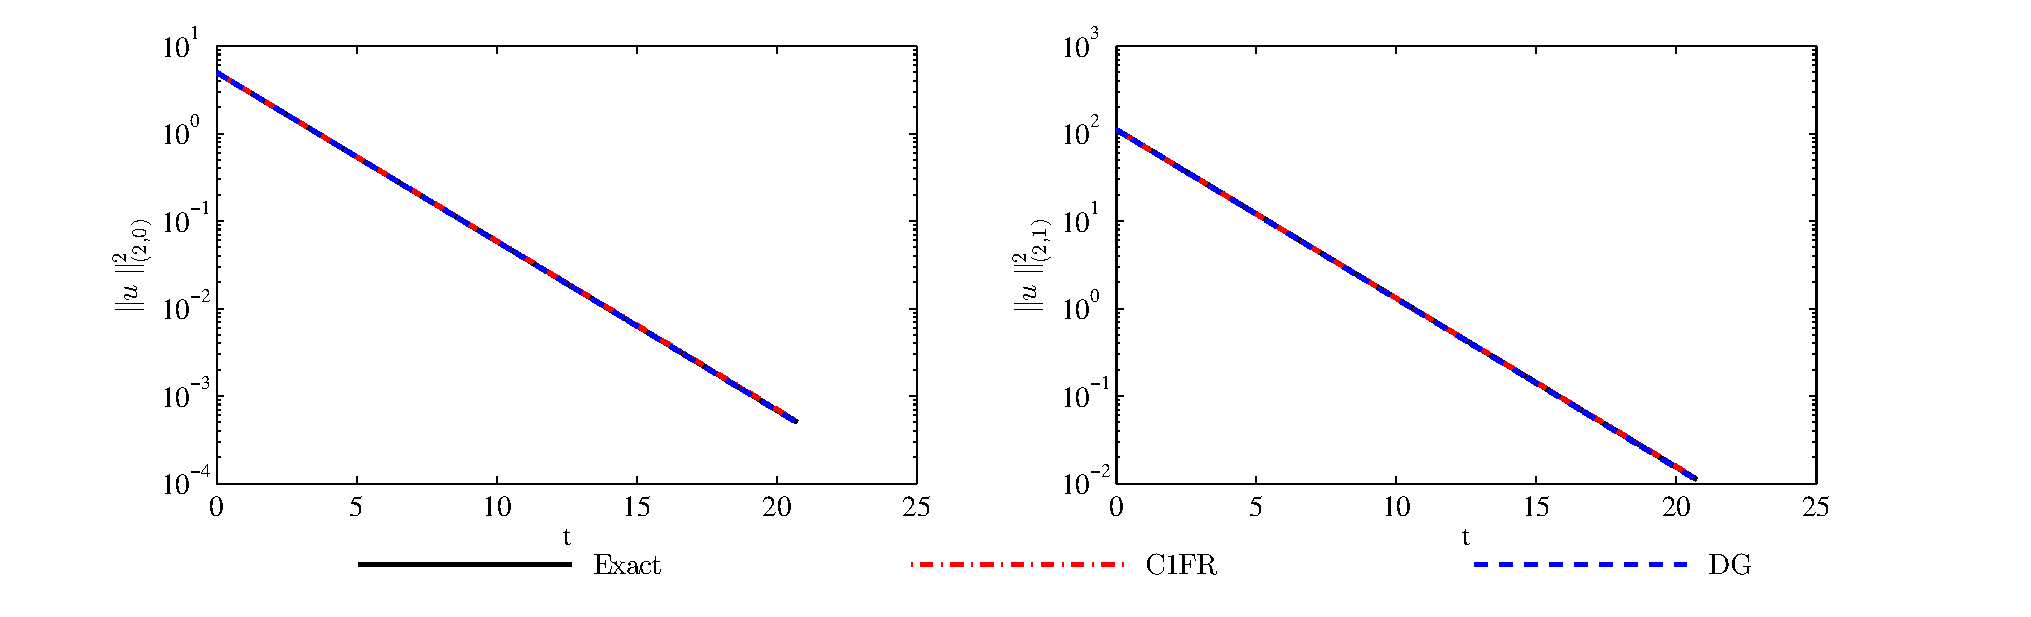
\includegraphics[width=1\textwidth,trim=\Ltrim cm 0cm \Rtrim cm 0cm]{\cmfrdir/Figures/Test_adv_diff/low_k}
\caption{Time history of norms of numerical solutions to the advection-diffusion equation and their first derivative. Initial condition is a sine wave with low wavenumber: $k = 0.25 (P+1)\pi/h$, $P = 3$, $h = 1$.}
\label{fig:low_wavenumber}
\end{figure}

\begin{figure}[h]
\centering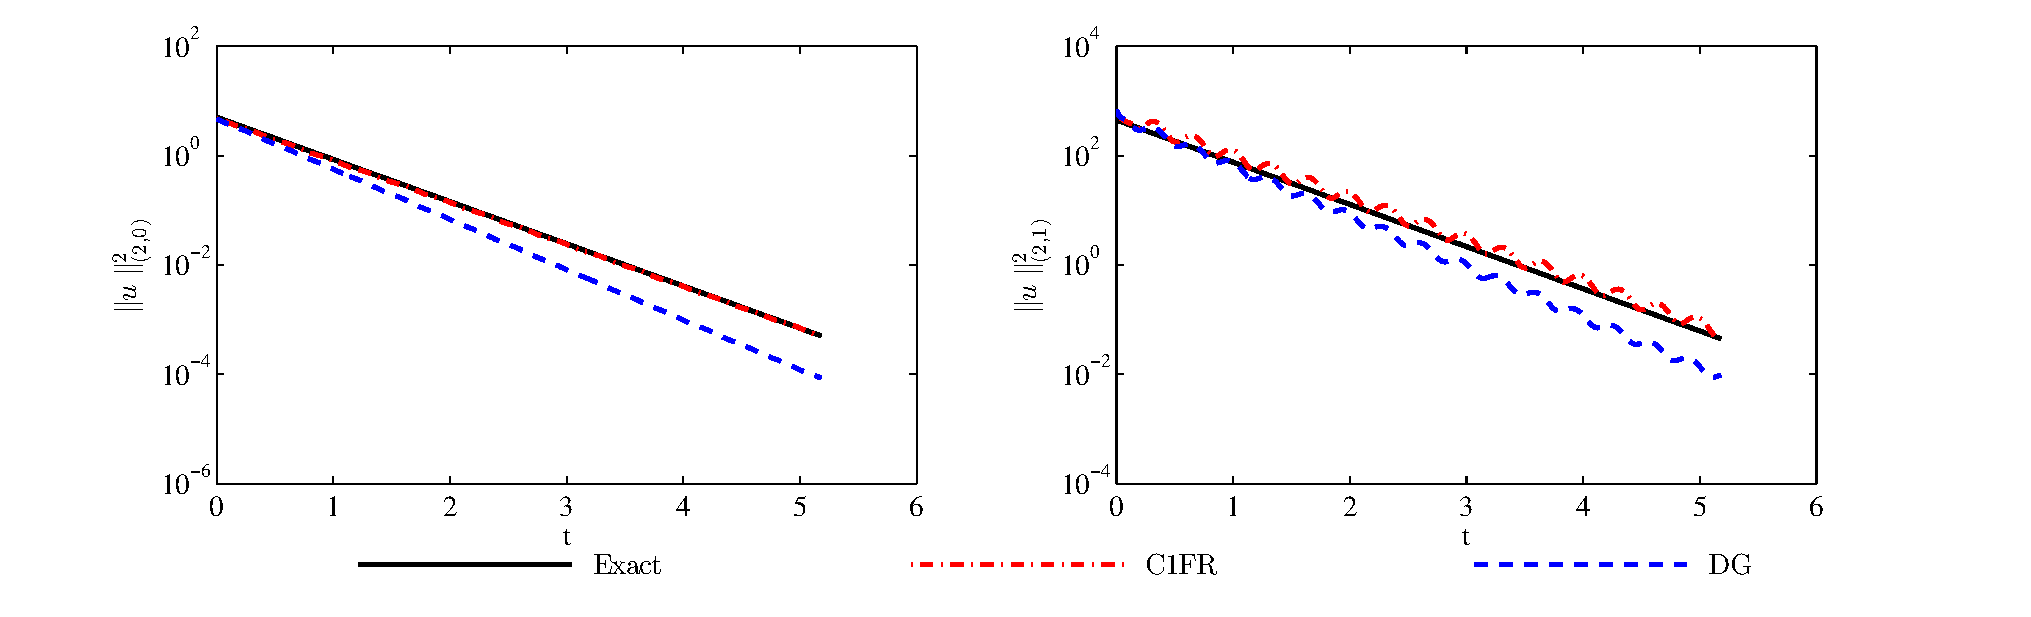
\includegraphics[width=1\textwidth,trim=\Ltrim cm 0cm \Rtrim cm 0cm]{\cmfrdir/Figures/Test_adv_diff/med_k}
\caption{Time history of norms of numerical solutions to the advection-diffusion equation and their first derivative. Initial condition is a sine wave with medium wavenumber: $k = 0.5 (P+1)\pi/h$, $P = 3$, $h = 1$.}
\label{fig:medium_wavenumber}
\end{figure}

\begin{figure}[h]
\centering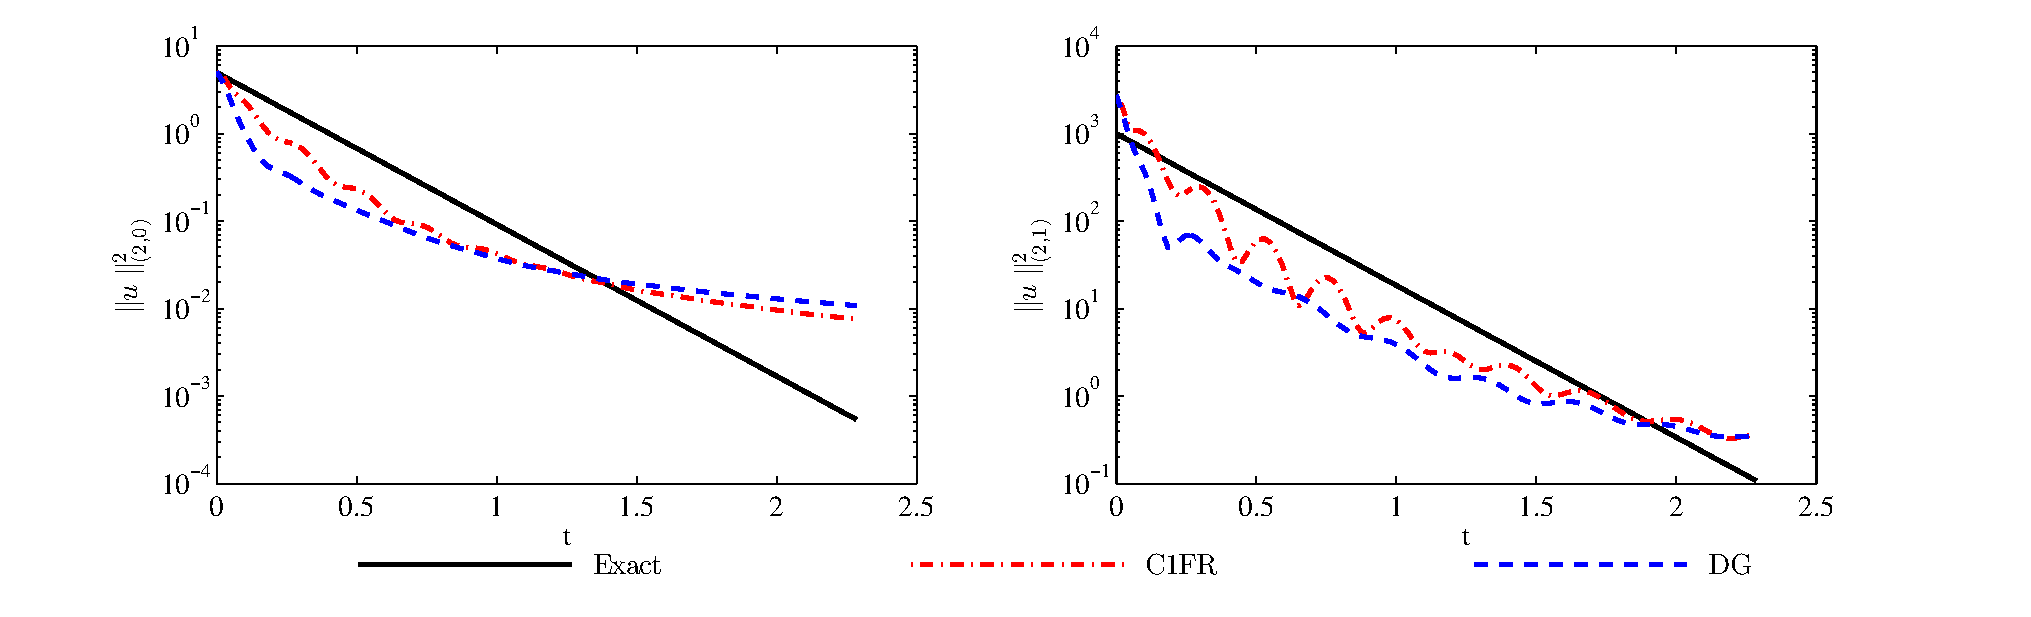
\includegraphics[width=1\textwidth,trim=\Ltrim cm 0cm \Rtrim cm 0cm]{\cmfrdir/Figures/Test_adv_diff/high_k}
\caption{Time history of norms of numerical solutions to the advection-diffusion equation and their first derivative. Initial condition is a sine wave with high wavenumber: $k = 0.75 (P+1)\pi/h$, $P = 3$, $h = 1$.}
\label{fig:high_wavenumber}
\end{figure}

%_ %_ %_ %_ %_ %_ %_ %_ %_ %_ %_ %_ %_ %_ %_ %_ %_ %
%\begin{figure}[h]
%\centering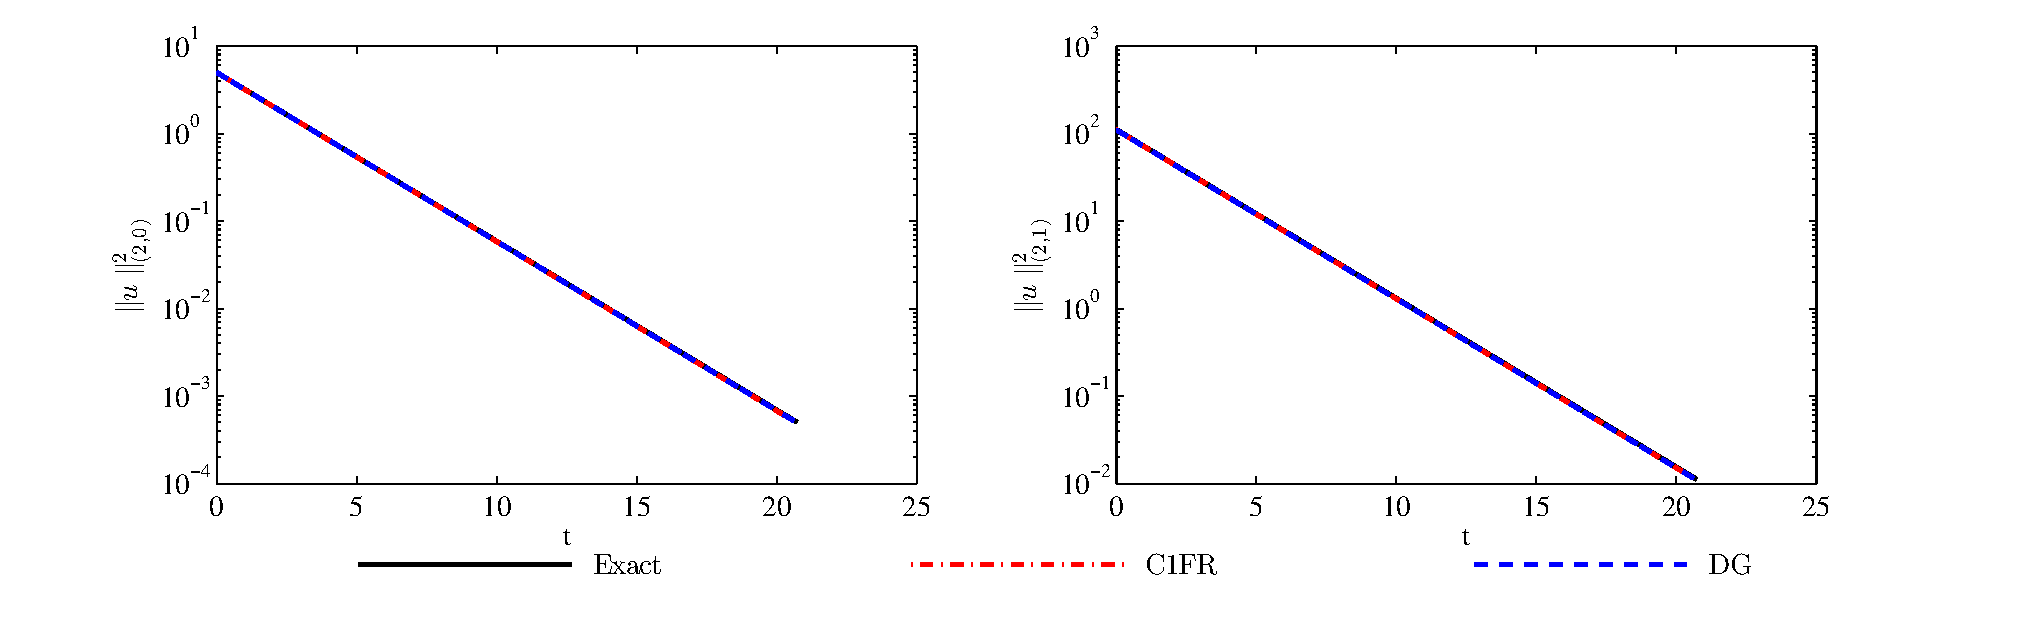
\includegraphics[width=1\textwidth,trim=\Ltrim cm 0cm \Rtrim cm 0cm]{Figures/Test_adv_diff/low_k_c_5e-3}
%\caption{Time history of norms of numerical solutions to the advection-diffusion equation and their first derivative. Initial condition is a sine wave with low wavenumber: $k = 0.25 (P+1)\pi/h$, $P = 3$, $h = 1$.}
%\label{fig:low_wavenumber2}
%\end{figure}
%
%\begin{figure}[h]
%\centering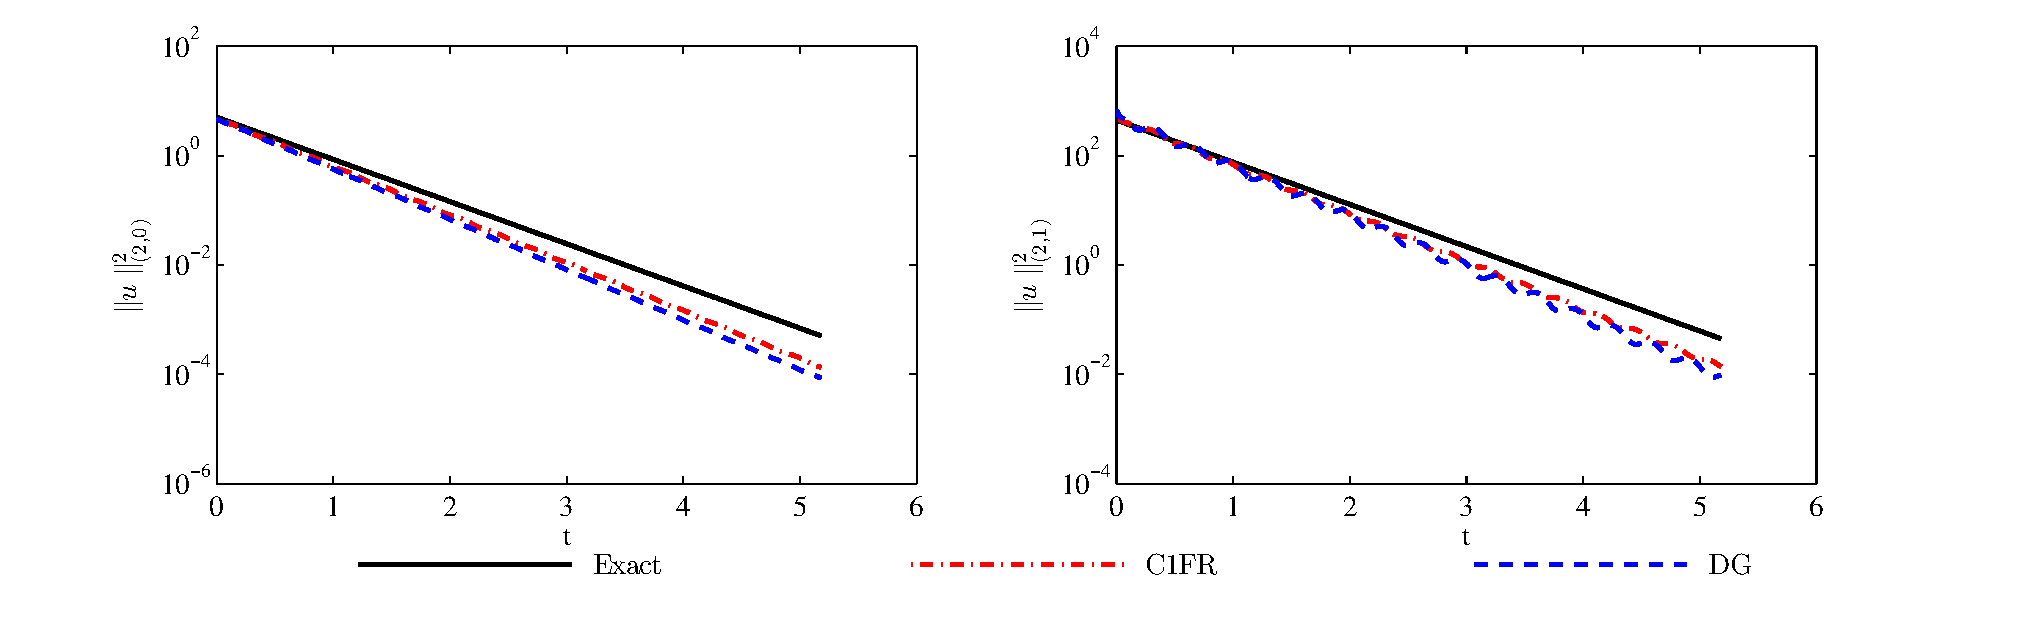
\includegraphics[width=1\textwidth,trim=\Ltrim cm 0cm \Rtrim cm 0cm]{Figures/Test_adv_diff/med_k_c_5e-3}
%\caption{Time history of norms of numerical solutions to the advection-diffusion equation and their first derivative. Initial condition is a sine wave with medium wavenumber: $k = 0.5 (P+1)\pi/h$, $P = 3$, $h = 1$.}
%\label{fig:medium_wavenumber2}
%\end{figure}
%
%\begin{figure}[h]
%\centering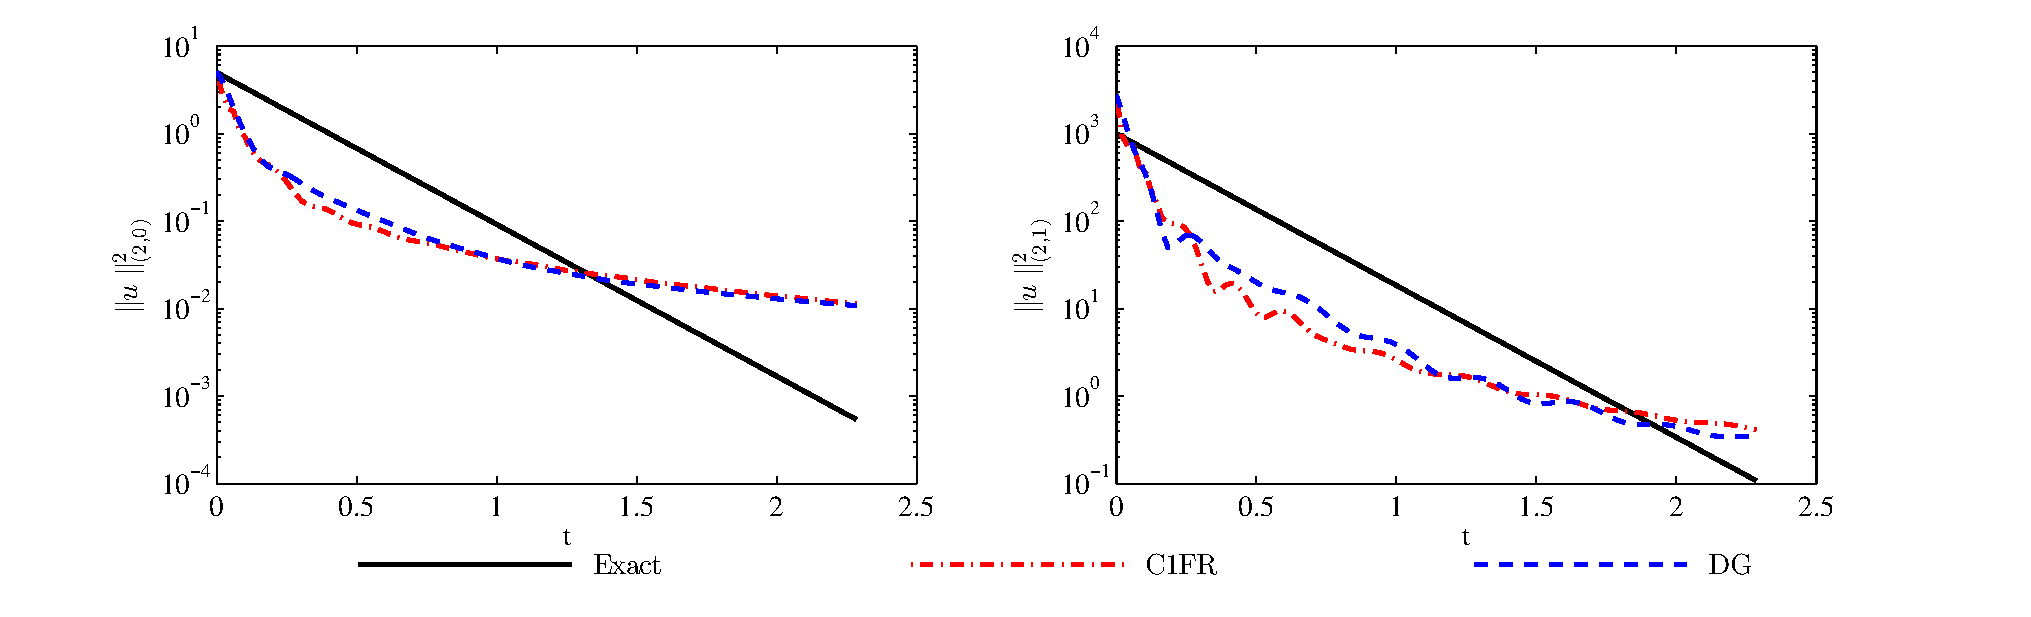
\includegraphics[width=1\textwidth,trim=\Ltrim cm 0cm \Rtrim cm 0cm]{Figures/Test_adv_diff/high_k_c_5e-3}
%\caption{Time history of norms of numerical solutions to the advection-diffusion equation and their first derivative. Initial condition is a sine wave with high wavenumber: $k = 0.75 (P+1)\pi/h$, $P = 3$, $h = 1$.}
%\label{fig:high_wavenumber2}
%\end{figure}

%_ %_ %_ %_ %_ %_ %_ %_ %_ %_ %_ %_ %_ %_ %_ %_ %_ %

%\begin{figure}
%\centering
%\subfigure[fig a]{\label{fig:high_wavenumber} 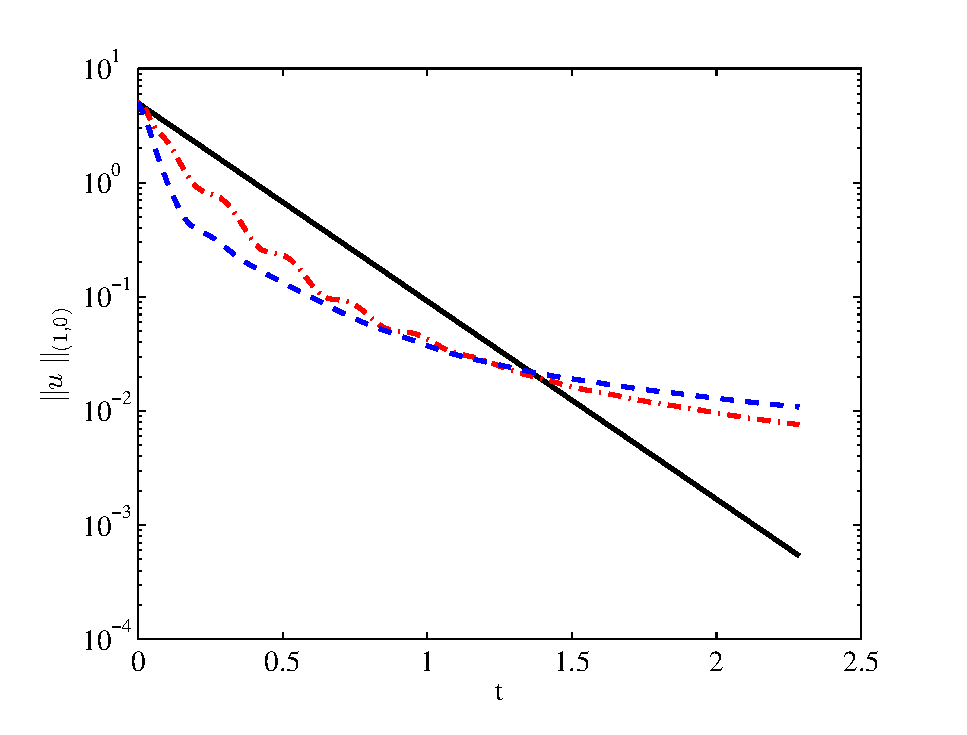
\includegraphics[width = .5\textwidth]{Figures/Test_adv_diff/eN0_high_k}
%\caption{energy history}}

%\end{subfig}
%\end{figure}

